\documentclass[../../thesis.tex]{subfiles}

\begin{document}
\begin{figure}[ht]
    \centering
    \pgfdeclarelayer{bg}    % declare background layer
    \pgfsetlayers{bg,main}  % set the order of the layers (main is the standard layer)
    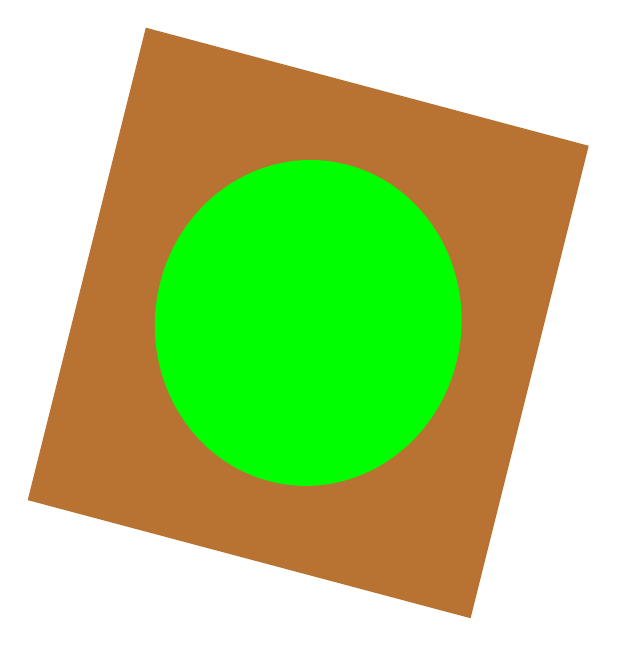
\begin{tikzpicture}
        \definecolor{copper}{rgb}{0.72, 0.45, 0.2}
        \tikzfading[name=fade out,
        inner color=transparent!0, outer color=transparent!100]
        \def\holerad{0.3}
        \def\factor{4}
        \def\xradius{2}
        \def\yradius{2/\factor}
        \def\height{1.05cm}
        \def\xandy{2 and 2/\factor}
            \tikzset{
          pics/.cd, %
          disc/.style ={
            code = {
              %% the foundation
              \path [fill=black!15] (-\xradius,0) -- (-\xradius,-\height) arc
              (180:360:\xandy) -- (\xradius,0) arc (0:180:\xandy);%
              \path [top color=black!25, bottom color=white, opacity=0.2] (0,0) ellipse
              [x radius=\xradius, y radius =\yradius];%
              \path [left color=black!25, right color=black!15] (-\xradius,0) --
              (-\xradius,-\height) arc (180:240:\xandy) -- +(0,\height) arc
              (240:180:\xandy);%
              \path [left color=black!15, right color=black!30] (\xradius,0) --
              (\xradius,-\height) arc (360:320:\xandy) -- +(0,\height) arc
              (320:360:\xandy);
              %% rays in front
              \foreach \col/\r/\shift/\stop/\opacity in {%
                black/205/25/20/100, %
                black/295/35/30/100, %
                black/295/30/30/200, %
                black/295/25/20/300, %
                white/245/14/14/100, %
                white/245/12/12/20, %
                white/245/10/10/10} {%
                \foreach \i [evaluate={\opposite=\r-180;}] in {0,1,...,\stop}{%
                  \fill [\col, fill opacity = 1/\opacity] (\opposite:0.1 and
                  0.1/\factor) -- (\r+\shift-\i:\xandy) -- ++(0,-\height) arc
                  (\r+\shift-\i:\r-\shift+\i:\xandy) -- +(0,\height) -- cycle; }}
              %% rays in back
              \foreach \r/\shift/\stop/\opacity in {%
                25/25/20/100, %
                115/35/3/150,%
                115/30/23/100} {%
                \foreach \i [evaluate={\opposite=\r-180;}] in {0,1,...,\stop}{%
                  \fill [black, fill opacity = 1/\opacity] (\opposite:0.1 and 0.1/\factor) --
                  (\r+\shift-\i:\xandy) arc (\r+\shift-\i:\r-\shift+\i:\xandy) --
                  cycle; }}
              %% masking the four edges in the center
              \foreach \i in {0.1, 0.2, ..., 0.4}%
              \fill[black!15, opacity=0.7, path fading=fade out]
              (0,0) ellipse[x radius=\i, y radius =\i/\factor];
              %% the light and the dark arcs
              \foreach \i [evaluate={\start=185+10*\i; \finish=355-10*\i;}]%
              in {0.1, 0.2, ..., 1.5}{%
                \draw[white, opacity=0.04, line width=\i, yshift=0.02cm]
                (\start:\xandy) arc (\start:\finish:\xandy);
                \draw[black!80, opacity=0.05, line width=\i, yshift=-\height]
                (\start:\xandy) arc (\start:\finish:\xandy); }
            }
          },%
          disc bottom/.style = {
            code = {
              \foreach \i/\opacity in {%
                1/20,2/20,3/20,4/30,5/35,6/40,7/60,8/80,9/100,10/100,11/100,12/100}%
                %\fill [red, fill opacity = 1/\opacity, yshift=-0.03cm] (0,-\height)
                ellipse [x radius = \xradius+\i/40, y radius = \yradius+\i/20/\factor];
              \path pic {disc};
            }
          },%
        }
        %
        \pgfdeclarelayer{bg}    % declare background layer
        \pgfsetlayers{bg,main}  % set the order of the layers (main is the
        \tikzmath{
        \l = 5.62;
        \h = 2.5;
        \d = 0.9;}
        % procces simages
        \begin{scope}[xslant= 0.25, yslant=-0.25]
            \filldraw[green] (3,3) circle (2);
            \begin{pgfonlayer}{bg}
                \fill[copper] (0,0) rectangle (6,6);
            \end{pgfonlayer}
        \end{scope}
    \end{tikzpicture}
    \caption{Membrane production}
    \label{fig:membrane production}
\end{figure}
\end{document}
